\chapter{Background}
\label{ch:background}

\section{Clustering}

\enquote{\emph{Clustering algorithms partition a given data set into several
groups based on some notion of similarity between objects.}}

A general class of methods to deal with unsupervised problems is clustering.
The most widely used is the \methodname{$k$-means algorithm}
\autocite{kmeans67}. After initially choosing $k$ centroids, an iterative
process takes place, divided in two phases. First each point is assigned to
the cluster of the closest centroid. Then centroids positions are updated by
taking the mean of all points belonging to their cluster. Convergence occurred
when centroids positions do not change anymore between iterations. In
practice, the algorithm is fast but it is only guaranteed to find a local
optimal of the within-cluster sum of squares: \[ \sum_{i=1}^{k} \sum_{ x_j \in
S_i} \left\| x_j - \mu_i \right\|^2 \] Another drawbacks is that $k$, the
number of clusters, has to be specified before algorithm execution, whereas
this information is often unknown at this stage. Finally, because it results
in a Voronoy diagram, the clusters found are linearly separable, which may not
reflect the actual data.

There are plenty of alternatives.

A cluster can be defined as an area of high density surrounded by low density
regions. This definition suggests to assign numerical value of density to
every point of space. A common method is \marginpar{Maybe there is a more
practical reference, especially for multivariate estimation}
\methodname{Kernel Density Estimation} \autocite{KDE56}. Basically, a kernel
is centered around each point (\ie{} a symmetrical weighting function, for
instance a Multivariate Gaussian) and the estimation of the probability
distribution $f$ is their normalized sum:
% http://en.wikipedia.org/wiki/Multivariate_kernel_density_estimation
\[ \hat{f}_\bold{h}(\bold{x})= \frac{1}{n} \sum_{i=1}^n K_\bold{h} (\bold{x} -
\bold{x}_i) \]

Yet this does not provide any clustering. One idea would to find the modes of
$\hat{f}$, which is the underlying principle of Mean Shift
\autocite{MeanShift95}. Another density based algorithm is \methodname{DBSCAN}
\autocite{DBSCAN96}. It has two parameters, a distance $\epsilon$ and a number
of points $\mathrm{minPts}$. A core sample is a point with at least
$\mathrm{minPts}$ neighbors in its $\epsilon$-neighborhood. From a core
sample, we visit all its neighbors to find other core samples belonging to the
same cluster. Once it is not more possible, we move to another point. Points
that are $\epsilon$ close to a core sample without having a large enough
neighborhood are also part of the cluster (but fringe points rather than
core). Any other remaining point is noise. With an appropriate index
structure, neighborhood queries takes $O(\log n)$ time and the algorithm runs
in $O(n\log n)$. Otherwise, one need to compute the pairwise distance matrix,
which takes $O(n^2)$ time and memory. DBSCAN find arbitrary number of clusters
with arbitrary shapes. In the special case where points carry user
identification (like photos or tweets), it can be tweaked to favor area that
features user diversity \autocite{PDBSCANKisilevich2010}.\marginpar{Explain
the principle}Another extension deals with cluster of varying density
\autocite{OPTICS99}.

\begin{comments}
	I didn't use these methods so maybe I don't need to talk about it\\
	Some are based on graphs. For instance \methodname{Spectral
	Clustering} \autocite{SpectralClustering01} (which is related to
	Kernel $k$-means, as shown by \textcite{KernelKmeans04}).
	\methodname{Affinity Propagation} \autocite{AffinityPropagation07}
% https://en.wikipedia.org/wiki/Affinity_propagation
% http://scikit-learn.org/stable/modules/clustering.html#affinity-propagation

	Other are hierarchical
\url{https://en.wikipedia.org/wiki/Hierarchical_clustering}
\end{comments}

A major component of all clustering algorithm is the distance function, and
the space where it operates. The default choice is the Euclidean metric in the
original feature space but these two parameters can be changed. In the latter
case, it often leads to dimensionality reduction.

\subsection{Dimensionality reduction}

Again, there are many methods, but many of them are based on the idea of
preserving distances between points, under the general name Multidimensional
Scaling \autocite{MDS77}. Given points $i$ and $j$ in the original space, we
know their separation $\delta_{i,j}$ with a weight $w_{i,j}$\footnote{that
denotes confidence in the measurement or importance of the points.}. We are
looking for their new position $x_i$ and $x_j$ in the reduced space such that
the stress \[ \sqrt{\frac{\sum w_{i,j}(\delta_{i,j} - d(x_i, x_j))^2}{\sum
d(x_i, x_j)^2}} \] is minimized. Instead of interpreting distances in a
geometrical sense, it is also possible to give a probabilistic fashion.
Namely, in Stochastic Neighbor Embedding \autocite{SNE02}, $d^2_{ij} =
\frac{\vnorm{x_i - x_j}^2}{\sigma^2_i}$  and $p_{ij} =
\frac{\exp(-d_{ij}^2)}{\sum_{k \neq i}\exp(-d_{ik}^2)}$ likewise $q_{ij} =
\frac{\exp(-\vnorm{y_i - y_j}^2)}{\sum_{k \neq i}\exp(-\vnorm{y_i - y_k}^2)}$
and we optimize $\sum_i KL(P_i || Q_i)$. In t-SNE \autocite{tSNE08}, better
distance modeling by a Student t-distribution with one degree of freedom
$q_{ij} = \frac{\left(1+\vnorm{y_i - y_j}^2\right)^{-1}}{\sum_{k \neq
i}\left(1+\vnorm{y_i - y_k}^2\right)^{-1}}$. A ingenious implementation runs
in $O(n\log n)$ \autocite{BarnesHut13}.

It is easier to visually evaluate clustering results in this two or three
dimensional space, although dimension are not necessarily meaningful.
Furthermore, it is justified by manifold recovering.

\subsection{Spatial data structure} kDtree and R-index. (see section 6 of LMNN
paper)

\section{Metric} \label{sec:metric}

\subsection{Ground metric}

Instead of projecting points in a new space, we can directly modify the norm
used to compute distance, that is replace the $L_2$ norm $\vnorm{x-y}_2^2$,
for instance by $L_1$ norm (Manhattan distance) or $L_\infty$. Noting that
$\vnorm{x-y}_2^2 = (x-y)^T A (x-y) = d_A(x,y)$, where $A=I$, one can also
replace $A$ by any positive definite matrix to still define a metric. A well
motivated choice is setting $A$ as the inverse of the covariance matrix,
corresponding to the Mahalanobis distance \autocite{Mahalanobis36}. But $A$
can be learned from the data in other semi-supervised ways, by specifying
constraints between pair of points. These constraints are based on class
labels, meaning we want points of the same class to be close and points of
different classes to be set apart. In this work, we consider two methods that
optimize $A$ subject to such pairwise constraints.

The first is \methodname{Information Theoretic Metric Learning}
\autocite{InfoMetric07}. Given a positive definite matrix $A$, we can
associate (up to a scaling constant) a multivariate Gaussian distribution of
mean $\mu$: $p(x; A) = \frac{1}{Z}\exp\left(-\frac{1}{2}d_A(x, \mu)\right)$.
We also need a reference matrix $A_0$ (for instance the identity or the
covariance matrix of the dataset), a set $S$ of similar points and a set $D$
of dissimilar points. We want $A$ to be close to $A_0$ in the sense of
relative entropy $\KL{p(x; A_0)}{p(x,A)} = \int \! p(x; A_0) \log\frac{p(x;
A_0)}{p(x; A)}\, \mathrm{d}x$ by solving
\begin{align*}
	\min_A &\quad \KL{p(x; A_0)}{p(x; A)} &\quad\\
	\text{subject to} &\quad d_A(x_i, x_j) \leq u &(i,j) \in S,\\
			  &\quad d_A(x_i, x_j) \geq l &(i,j) \in D.
\end{align*}

The other one is \methodname{Large Margin Nearest Neighbor} \autocite{LMNN09}
\begin{figure}[ht]
	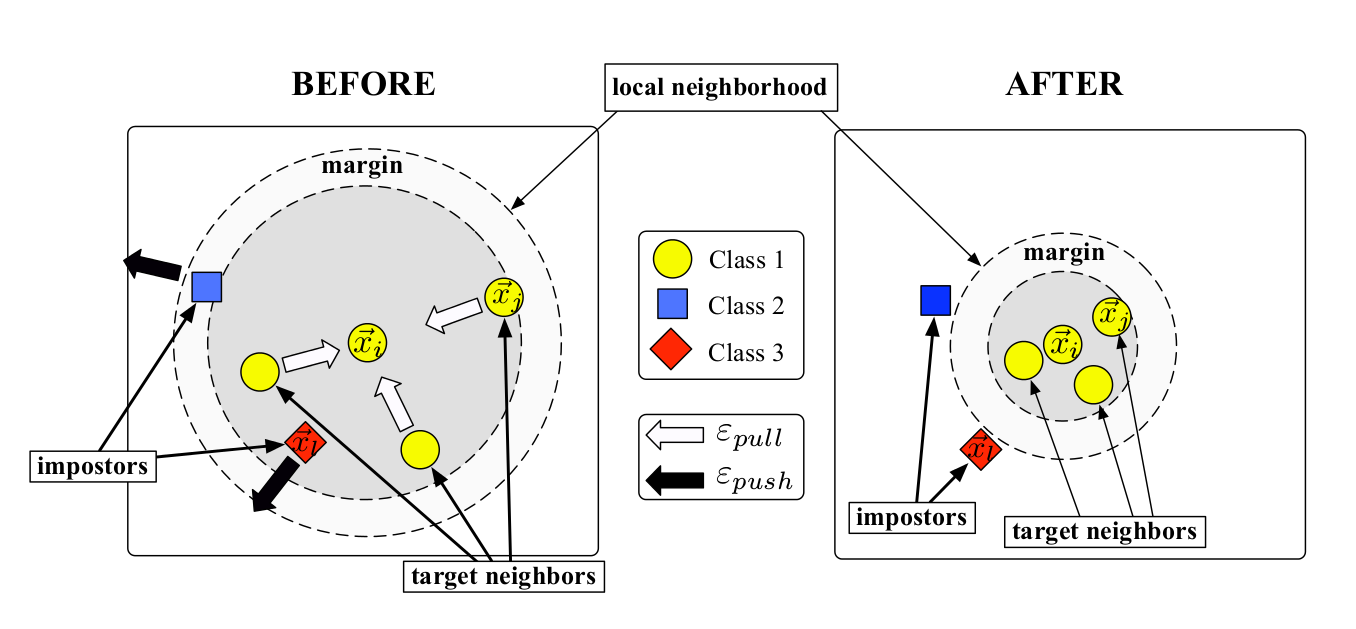
\includegraphics[width=\textwidth]{schema_lmnn}
	\caption{Neighborhood of a point, from \autocite{LMNN09}.\label{fig:lmnn}}
\end{figure}
$N_i$ is the set of the $k$ closest neighbors of $x_i$ in the
original space which share the same class, called target neighbors. Closer
points of different class are impostors (see \autoref{fig:lmnn}
\vpageref{fig:lmnn}). The optimization pushes target neighbors close to $x_i$
while pulling away impostors.  The number of active constraints is linear
rather than quadratic because only the neighborhood of each points contribute
to it. Thus the semidefinite program can be solved efficiently.
\begin{equation}
	\min_A \sum_{i, j\in N_i}
	\underbrace{d_A(x_i, x_j)}_\text{\emph{pull} target neighbor $x_j$ closer} +
	\underbrace{\mu \sum_{k, y_k\neq y_i} \left[ 1 + d_A(x_i, x_j) -
	d_A(x_i, x_k)\right]_+}_\text{\emph{push} impostor $x_k$ beyond target
	neighbor $x_j$}
\end{equation}
where $[x]_+$ is the hinge-loss: $[x]_+=\max(0, x)$

The end result is a linear, global metric but there are other approaches. One
can learn multiple local metrics, or a non linear metric like
\methodname{Gradient Boosting LMNN} \autocite{GBLMNN11} \emph{same formulation
but distance in a mapping space and the mapping is learned by a pool a weak
learner}.

A more complete overview of metric learning is given in the survey of
\textcite{MetricSurvey13}.

\subsection{Set metric} We discussed metrics between points but in this work,
we also used distances between set of such points.

geometric: For instance, the bottleneck distance \autocite{Bottleneck96} (the
smallest distance between pairs of farthest point), the sum of the distance of
each point to its closest neighbor, or the Hausdorff distance (the largest
distance between pairs of closest point) and its variation
\autocite{ModifiedHausdorff94}.

Assignment problem and Hungarian algorithm $O(n^4)$ and $O(n^3)$
\autocite{Hungarian57}. Transportation problem. Because these problem have min
cost flow constraints matrix, they are totally unimodular (\ie{} every non
singular sub square matrix has a determinant of $+1$ or $-1$) and thus admits
a integer solution.  It may be more convenient to consider non integer supply
and demand, which leads to fractional weight and probabilistic interpretation.
For instance the modern Kantorovitch formulation of the Transportation
problem: $\underset{\gamma \in \Gamma(\mu, \nu)}{\mathrm{inf}} \int_{X\times
Y} c(x,y)\mathrm{d}\gamma(x,y)$. It is related to the Wasserstein distance of
two probability measures $\mu$ and $\nu$ of a space $M$ with
$p$\textsuperscript{th} finite moment $W_p(\mu, \nu) = \left( \underset{\gamma
\in \Gamma(\mu, \nu)}{\mathrm{inf}} \int_{M\times M}
d(x,y)^p\mathrm{d}\gamma(x,y)\right)^{\frac{1}{p}}$. $W_1$ is also called
\methodname{Earth Mover's Distance} \autocite{EMD98}.


An lower-complexity algorithm using L1 ground metric. Code is available and
they claim 100x speed up for 2D histograms \autocite{Ling2007}

The approximation is based on wavelet but the complexity is exponential with
the number of dimension so it's probably infeasible for d>6
\autocite{Shirdhonkar2008}

The assumption here is that there is upper bound on the distance between
points. They also exhibit nice speed-ups and code is available.
\autocite{Pele2009}

It computes lower and upper bounds of EMD quickly, with GPU and in parallel.
The author also claims that the distance performs better for classification
task. Code is available but looking at it and reading the paper, it seems to
work only in one dimension. \autocite{FastEMD13}

% ground metric learning for EMD? \autocite{LearnEMD14}

information theoretic distance over some probability distributions, like the
Kullback--Leibler divergence or a metric based on it, like the
\methodname{Jensen--Shannon Divergence} \autocite{JensenShannon03}.
